% -*- coding: utf-8 -*-
%%%%%%%%%%%%%%%%%%%%%%%%%%%%%%%%%%%%%%%%%%%%%%%%%%%%%%%%%%%%%%%%%%%%%%%%%%%%%%%%
%2345678901234567890123456789012345678901234567890123456789012345678901234567890
%        1         2         3         4         5         6         7         8

%\UseRawInputEncoding


\documentclass[letterpaper, 10 pt, conference]{ieeeconf}  % Comment this line out if you need a4paper

%\pdfminorversion=4              % tell pdflatex to generate PDF in version 1.4
\usepackage[T1]{fontenc}
\usepackage{amssymb}
\usepackage{graphicx}
\usepackage{placeins}
\usepackage{multicol}
\usepackage{subcaption}
\usepackage{mathtools}
\usepackage{multirow,makecell}
\usepackage{caption}
\usepackage{xcolor}

%\documentclass[a4paper, 10pt, conference]{ieeeconf}      % Use this line for a4 paper

\IEEEoverridecommandlockouts                              % This command is only needed if 
                                                          % you want to use the \thanks command

\overrideIEEEmargins                                      % Needed to meet printer requirements.

%In case you encounter the following error:
%Error 1010 The PDF file may be corrupt (unable to open PDF file) OR
%Error 1000 An error occurred while parsing a contents stream. Unable to analyze the PDF file.
%This is a known problem with pdfLaTeX conversion filter. The file cannot be opened with acrobat reader
%Please use one of the alternatives below to circumvent this error by uncommenting one or the other
%\pdfobjcompresslevel=0
%\pdfminorversion=4

% See the \addtolength command later in the file to balance the column lengths
% on the last page of the document

% The following packages can be found on http:\\www.ctan.org
%\usepackage{graphics} % for pdf, bitmapped graphics files
%\usepackage{epsfig} % for postscript graphics files
%\usepackage{mathptmx} % assumes new font selection scheme installed
%\usepackage{times} % assumes new font selection scheme installed
%\usepackage{amsmath} % assumes amsmath package installed
%\usepackage{amssymb}  % assumes amsmath package installed
\usepackage{cite}

\title{\LARGE \bf
RO-Net: Recurrent Neural Networks for Range-only SLAM using range-only measurements}


\author{Hyungtae Lim$^{1}$ , Junseok Lee$^{1}$, Changgyu Park$^{1}$, Ye Eun Kim$^{1}$, % <-this % stops a space
\thanks{$^{1}$Hyungtae Lim, $^{1}$Junseok Lee, $^{1}$Changgyu Park, and $^{1}$Ye Eun Kim are with
	the Urban Robotics Laboratory, Korea Advanced Institute of Science
	and Technology (KAIST) Daejeon, 34141, South Korea. {\tt\small \{shapelim, ljs630, cpark, yeeunk\}@kaist.ac.kr}}%
%
}


\begin{document}

\captionsetup[figure]{labelformat={default},labelsep=period,name={Fig.}}


\maketitle
\thispagestyle{empty}
\pagestyle{empty}


%%%%%%%%%%%%%%%%%%%%%%%%%%%%%%%%%%%%%%%%%%%%%%%%%%%%%%%%%%%%%%%%%%%%%%%%%%%%%%%%
\begin{abstract}

Range-only(RO) SLAM is a method for localizing a mobile robot and beacons by mainly utilizing distance measurements. Because range-only measurements have only magnitude so it has rank-deficiency. And distance is only measured by the \textcolor{red}{time of flight(TOF)}, data is noisy.

In this paper, we proposed a novel approach to range-only SLAM using multimodal bidirectional stacked LSTM models. Unlike the traditional probability-based range-only SLAM method, we present a novel approach using a recurrent neural network architecture that directly learns the end-to-end mapping between distance data and robot position.

We gathered our own dataset and tested in 2 cases exploiting eagle eye motion capturer camera. The multimodal bidirectional stacked LSTM structure exhibits the precise estimates of robot positions, but one case, it is less accurate than traditional SLAM algorithm. 


\end{abstract}


%%%%%%%%%%%%%%%%%%%%%%%%%%%%%%%%%%%%%%%%%%%%%%%%%%%%%%%%%%%%%%%%%%%%%%%%%%%%%%%%
\section{INTRODUCTION}

 
 \textcolor{red}{SLAM is widely used in autonomous vehicles, drones, intelligence field robots, and mobile phone applications. Thus, according to the smart city development plan, several technologies are required, and the importance and the necessity of SLAM are increasing together. Various kinds of sensors are utilized to SLAM, such as GPS, LiDAR, ultrasonic-based sensor, camera and distance sensor.Trilateration is a conventional algorithm for locating a vehicle in the metropolitan area by range measurements between the vehicle and fixed beacon sensors} \cite{staras1972accuracy}. Due to the convenience of trilateration that estimates the position of a receiver of range sensors if one only knows range measurement, trilateration algorithm has been widely incorporated into robotics fields, especially utilized in the indoor environment to estimate the position of an object by distance measurements obtained from range sensors such as UWB, ultrasonic, laser-based beacon sensors \cite{thomas2005revisiting, cho2010mobile,raghavan2010accurate}. Specifically, range-only Simultaneous Localization and Mapping(RO-SLAM) methods are utilized popularly, which not only estimate the position of the receiver of range sensors, but also localize the position of range sensors regarded as features on a map, and studies have been conducted continuously in terms of probability-based approach\cite{blanco2008pure, blanco2008efficient,fabresse2013undelayed, shetty2018particle}.
 
 In the meantime, as deep learning age has come\cite{lecun2015deep}, various kinds of deep neural architectures have been proposed for many tasks related to robotics field, such as detection\cite{lenz2015deep,cai2016unified, smith2018object}, navigation\cite{zhu2017target, hamandi2018deepmotion}, pose estimation\cite{walch2017image}, and so on. Especially, recurrent neural networks (RNNs), originated from Natural Language Process(NLP) area\cite{elman1990finding}, have been shown to achieve better performance in case of dealing with time variant information, thereby RNNs are widely utilized such as not only speech recognition, but also pose estimation and localization\cite{walch2017image, gladh2016deep, wang2017deepvo, kendall2015posenet, turan2018deep}. 
 
 In this paper, we propose a deep learning-based SLAM method by multimodal stacked bidirectional Long Short-Term Memory(multimodal stacked Bi-LSTM) for more accurate localization of the robot. Using deep learning, our structure directly learns the end-to-end mapping between range measurements and robot position. This operation non-linearly maps the relationship not only considering the long-range dependence of sequential distance data by the LSTM, but also using the correlation of the backward information and the forward information of the sequence of each time step by virtue of its bidirectional architecture. \textcolor{red}{Existing RO SLAM needs calibration before filtering, and then, range measurement undergoes outlier rejection, prediction and correction processes are needed.	Furthermorme, it uses low dimensional data to perform localization, there is a disadvantage that estimation is difficult even if the value deviates slightly from the model.} \textcolor{green}{Therefore, we solve this complex algorithm with end-to-end based deep learning. This system overview is shown in the figure below.}
 
\begin{figure}[h]
	
	\centering
	%\subfigure[]{
		%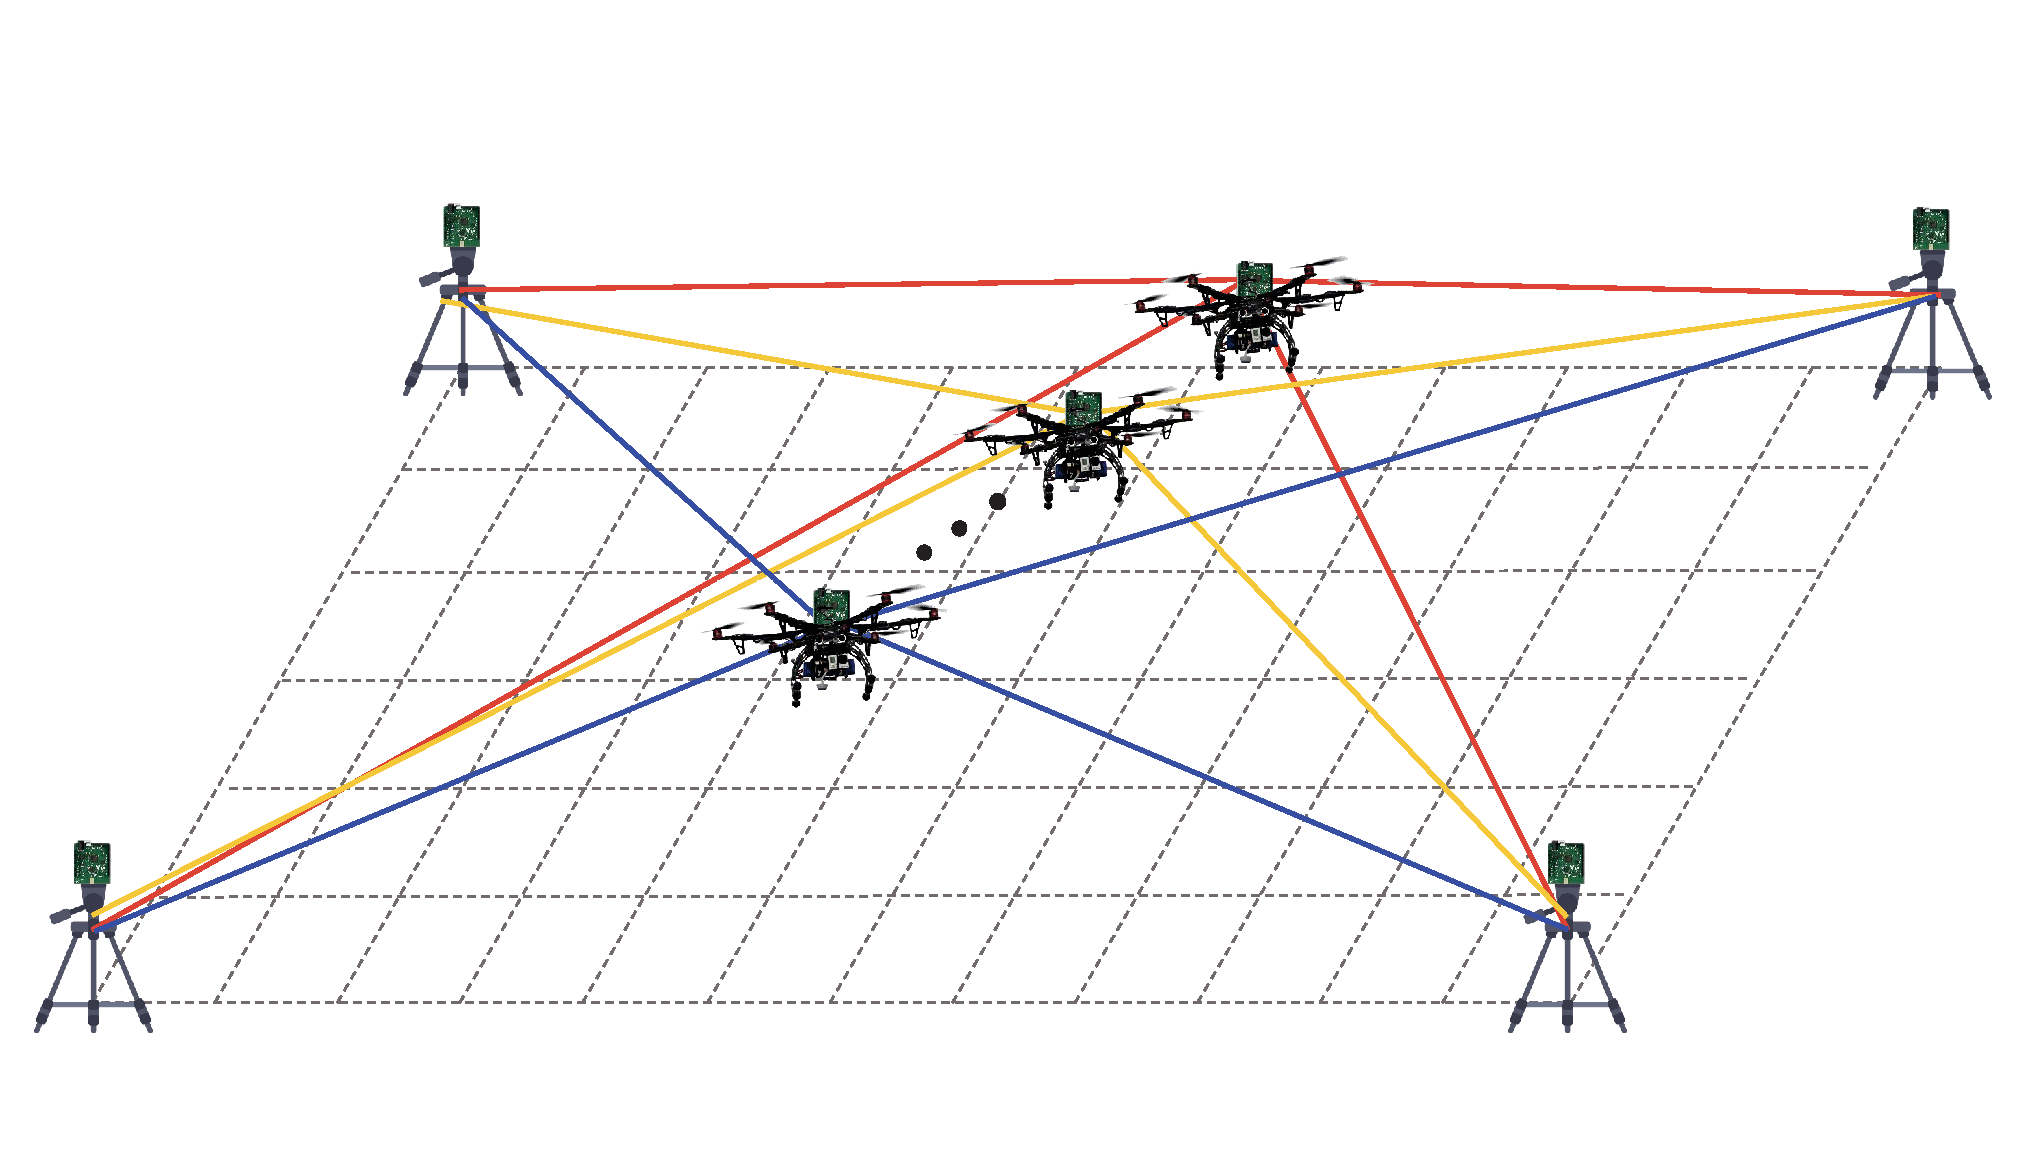
\includegraphics[height=4.5cm]{Drone_image_1}
	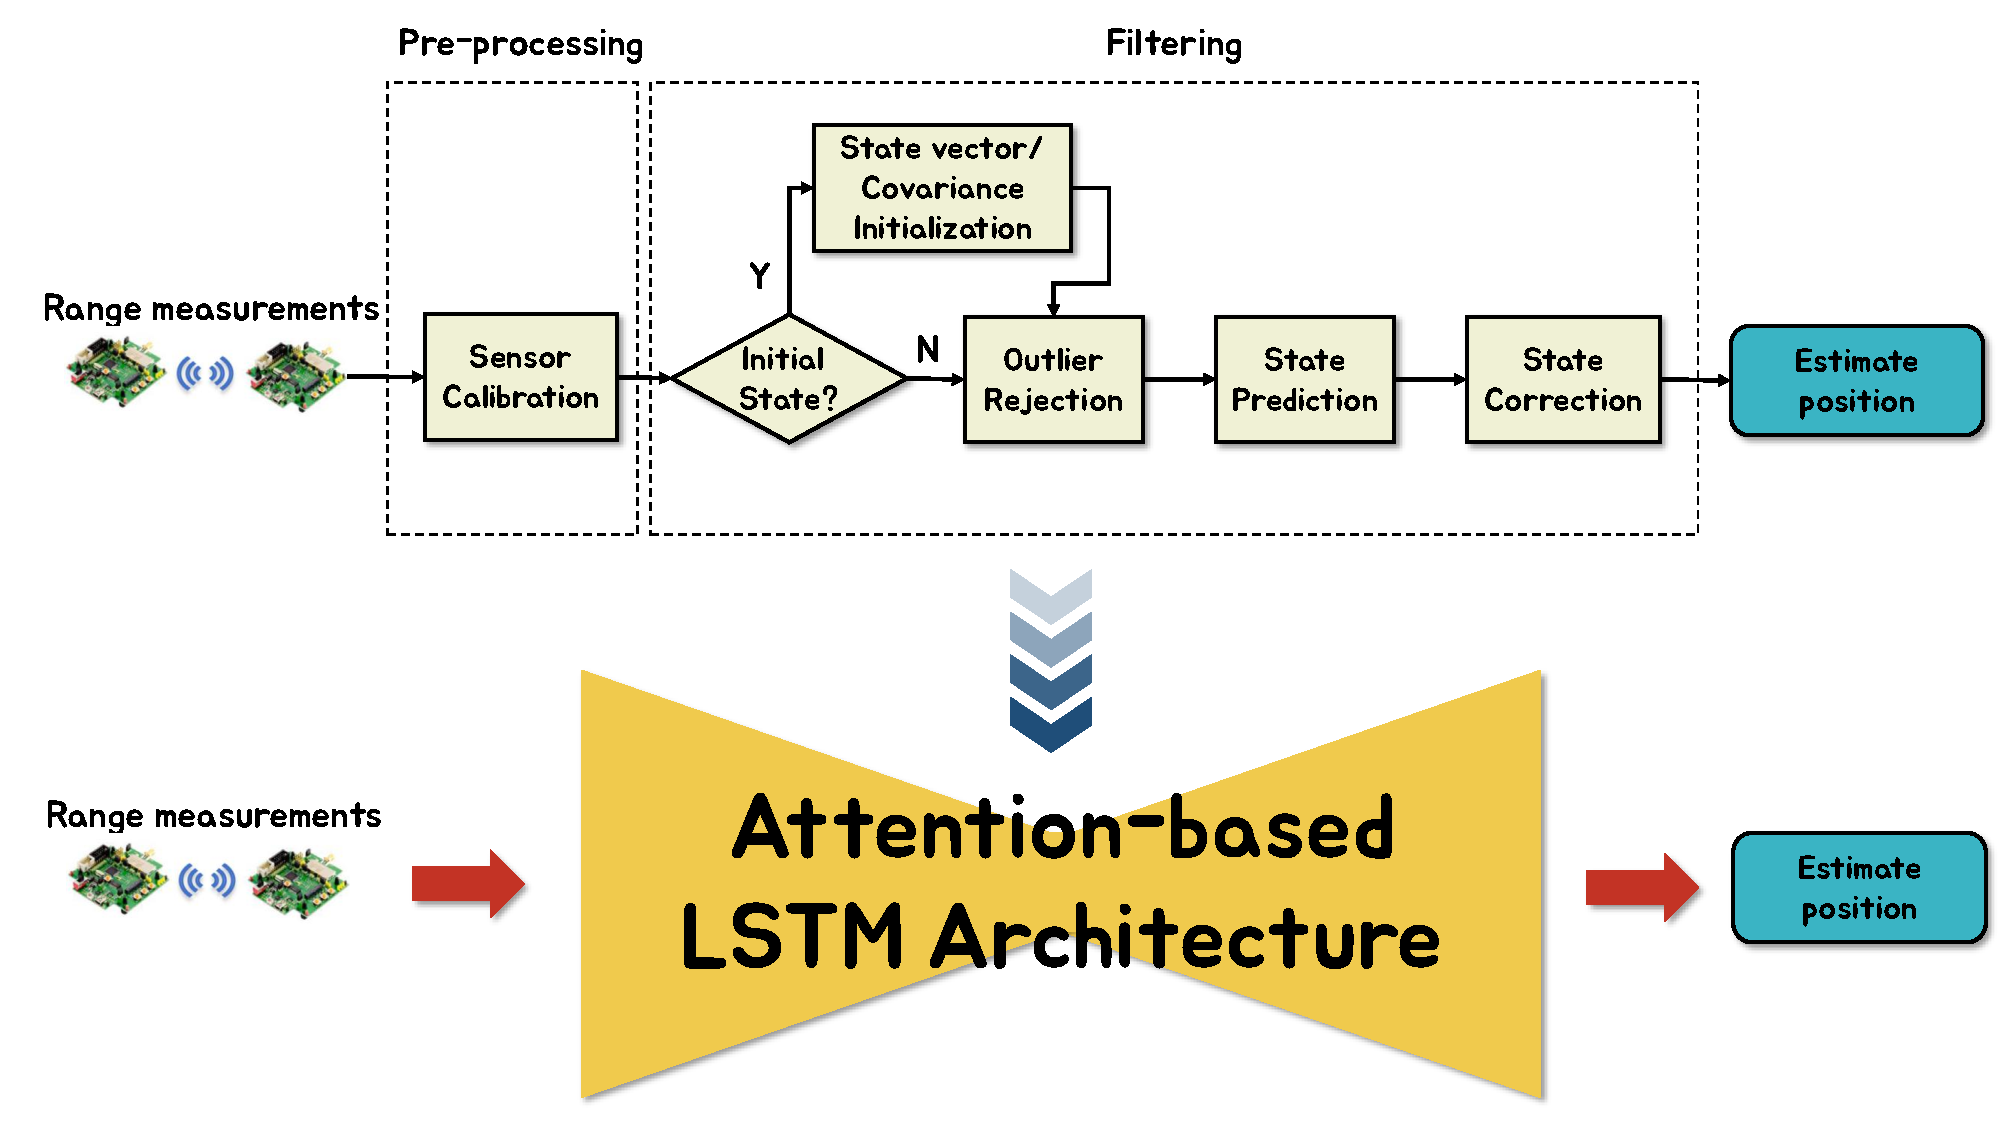
\includegraphics[height=5cm]{CE554_traditional_to_RNN}
	\label{fig:example}
	\caption{System overview. A robot localizes its own pose through distance data and the derivative of distance data. }
	
\end{figure}

\section{Related Works}

In this section, we briefly survey previous researches closely focused on 
RO-SLAM, Long Short-Term Memory(LSTM) model and applications of LSTMs to solve domain problems.

\subsubsection{RO-SLAM}


\textcolor{red}{SLAM is a technique for building the map information while localizing the position of the robot while moving. Localization of the SLAM predicts the current position of the robot using the landmark measured by the sensor, and mapping locates the terrain object based on the pose of the robot. Research on this technology has been actively carried out, and researches and techniques have been summarized.}In 2006, the ad doc sensor network consisting of range detection beacon was applied to SLAM technology for various ranges. This technology integrates node-to-node measurements to reduce drift and expedite node-map convergence \cite{djugash2006range} In 2008, the technique to consistently combine the observation information considering the uncertainty was studied through comparing the experimental data with the actual robot and simulation using Ultra Wide-Band (UWB) devices and Rao-Balckwellized Particle Filter (RBPF) \cite{blanco2008pure}.  In 2012, a simple and efficient algorithm for position recognition with high accuracy and low computational complexity was researched with ultrasonic sensors \cite{yang2012efficient}. In recent years, 3-dimensional-based SLAM has also been under active research and development. In 2013, a localization mapping approach of a wireless sensor network (WSN) node was studied through a centralized EKF-SLAM-based optimization research \cite{fabresse2013undelayed}. In addition, in 2014, a method of minimizing noise and localizing Unmanned Aerial Vehicle (UAV) by using  range-only measurement while simultaneously mapping the position of the wireless range sensors were proposed \cite{fabresse2014robust}. 
SLAM based on range measurement has been continuously researched and developed then applied to various fields. In this paper, we propose a novel technology that applying deep-learning to range-only SLAM that derives accurate range and robot position measurement through in-depth learning. 


\subsubsection{LSTM}

LSTM is a type of Recurrent Neural Networks(RNNs) that has loops so that infer output based on not only the input data, but also the internal state formed by previous information. In other words, while the RNN deals with sequential data, the network has remembered the previous state generated by past inputs and might be able to output the present time step via internal state and input, which is very similar to filtering algorithms.

However, RNNs often have a \textit{vanishing gradient problem},i.e., RNNs fail to propagate the previous matter into present tasks as time step gap grows by. In other words, RNNs are not able to learn to store appropriate internal states and operate on long-term trends. That is the reason why the Long Short-Term Memory (LSTM) architecture was introduced to solve this long-term dependency problem and make the networks possible to learn longer-term contextual understandings\cite{hochreiter1997long}.
By virtue of the LSTM architecture that has memory gates and units that enable learning of long-term dependencies\cite{zaremba2014learning}, LSTM are widely used in most of the deep learning research areas and numerous variations of LSTM architecutres have been studied.

\begin{figure*}[ht]
	
	\centering
	%\subfigure[]{
	%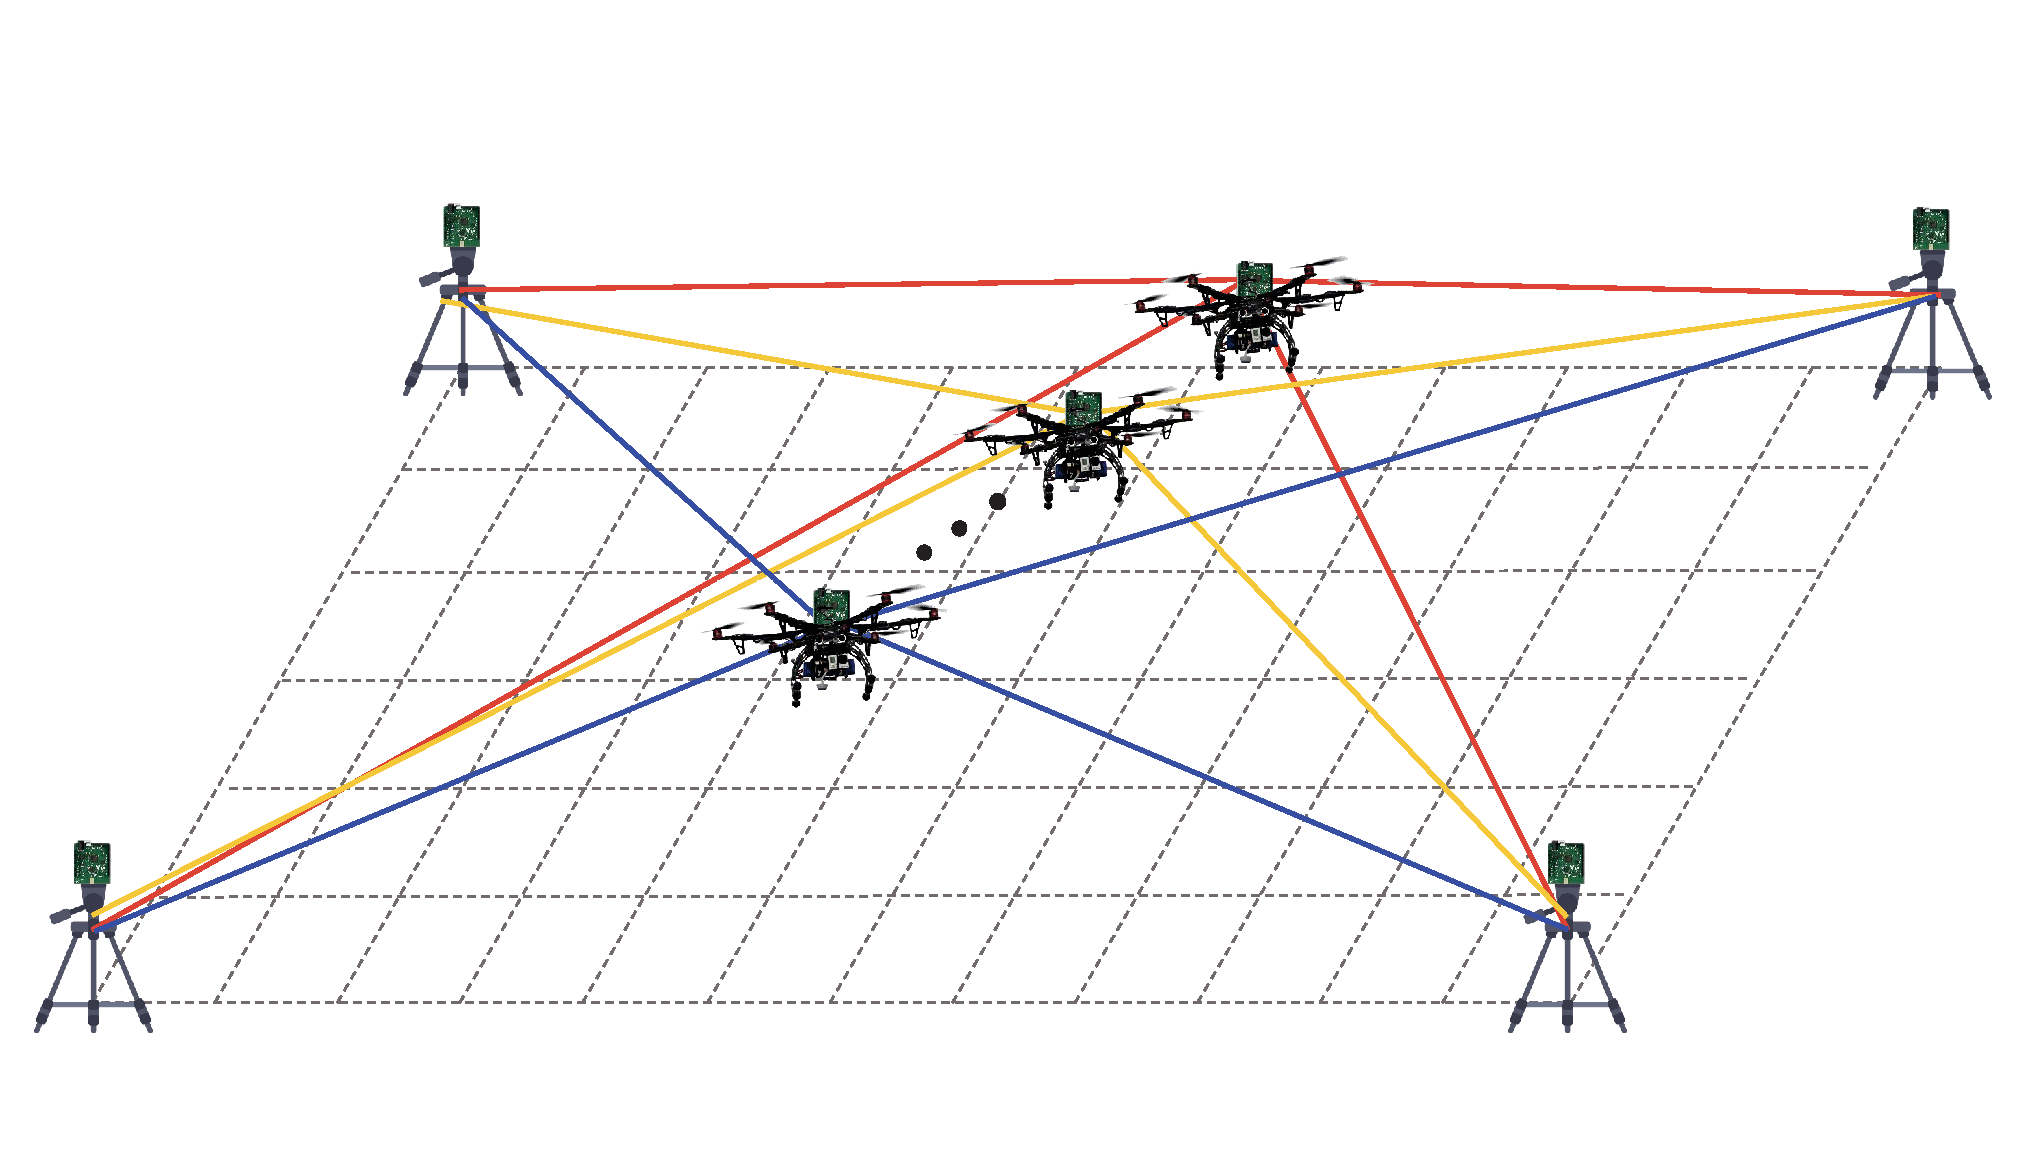
\includegraphics[height=4.5cm]{Drone_image_1}
	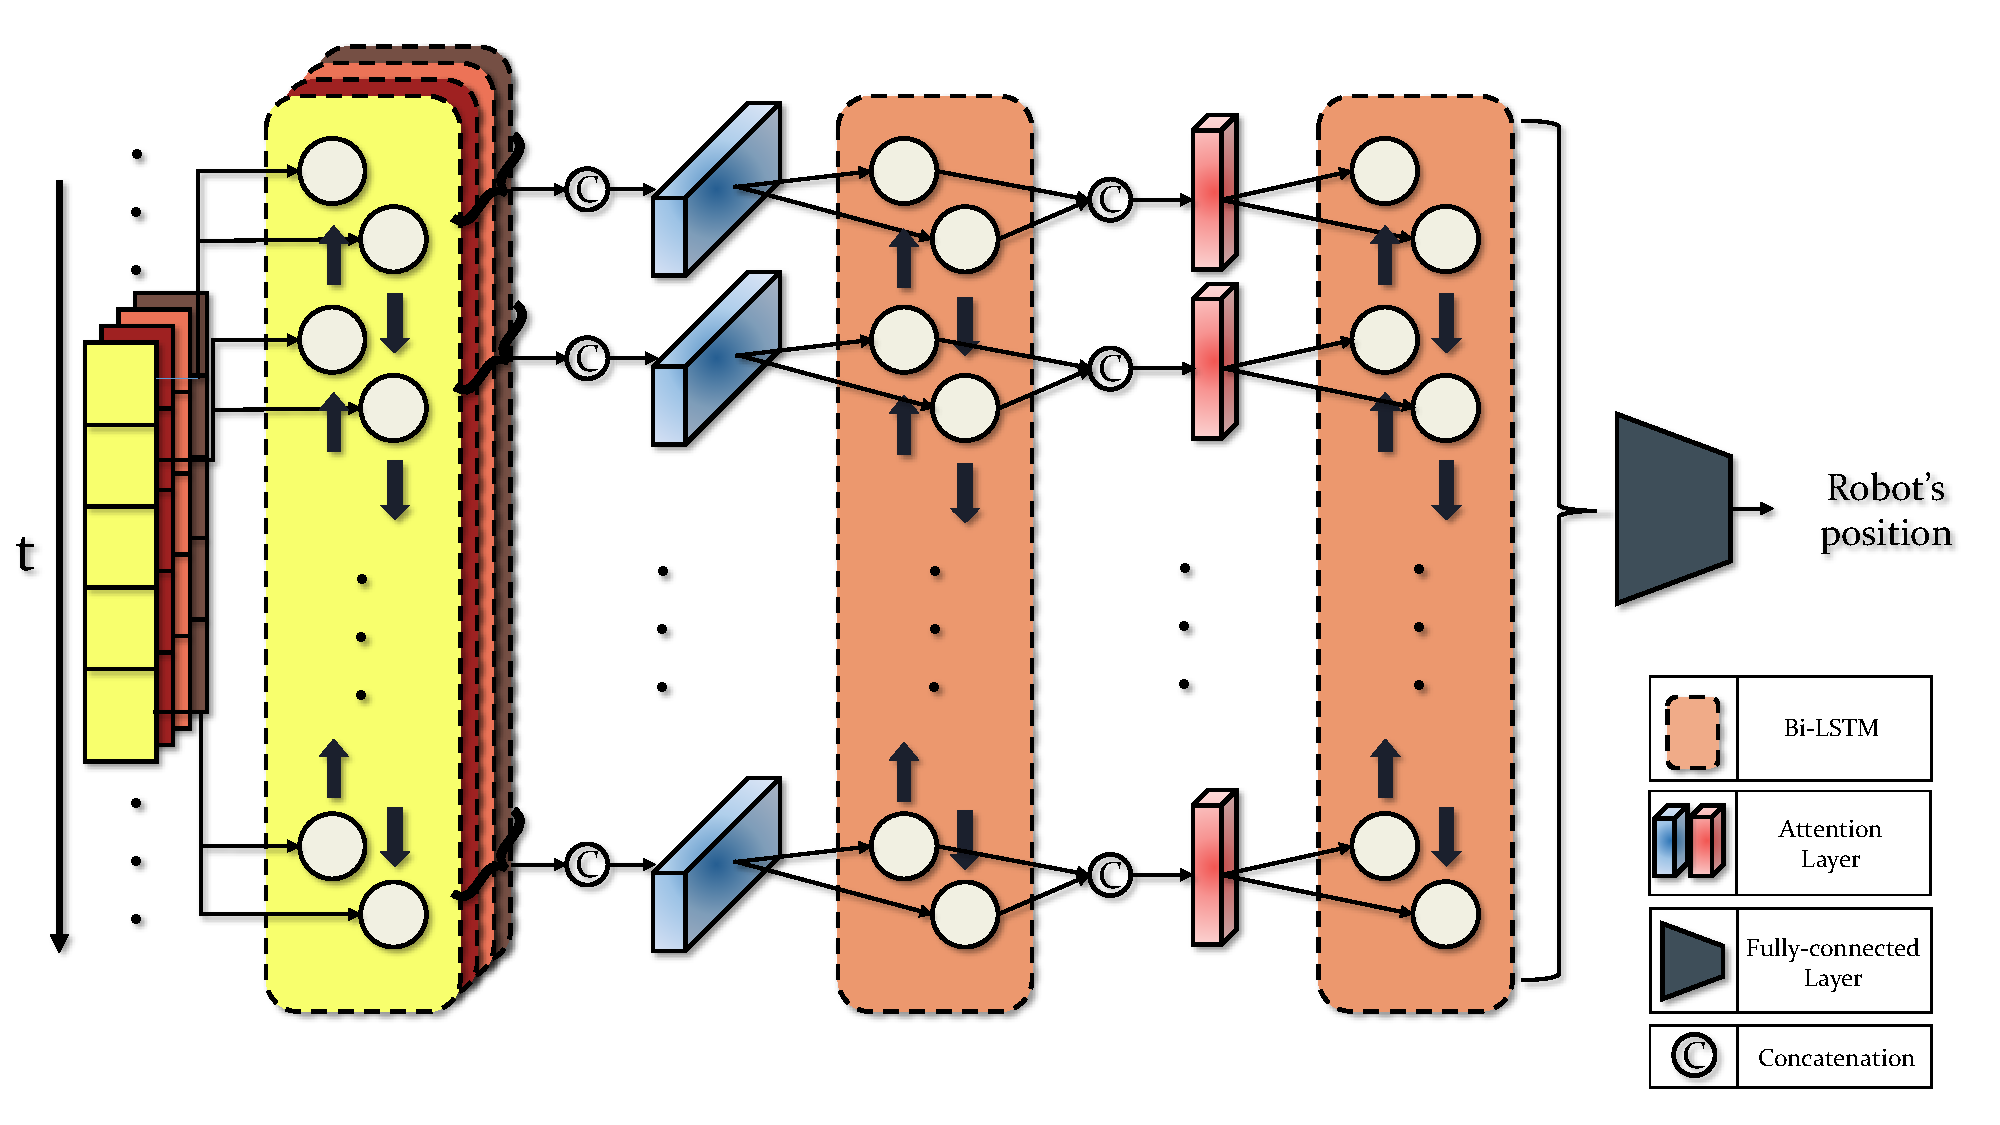
\includegraphics[height=10 cm]{CE554_networks}
	
	%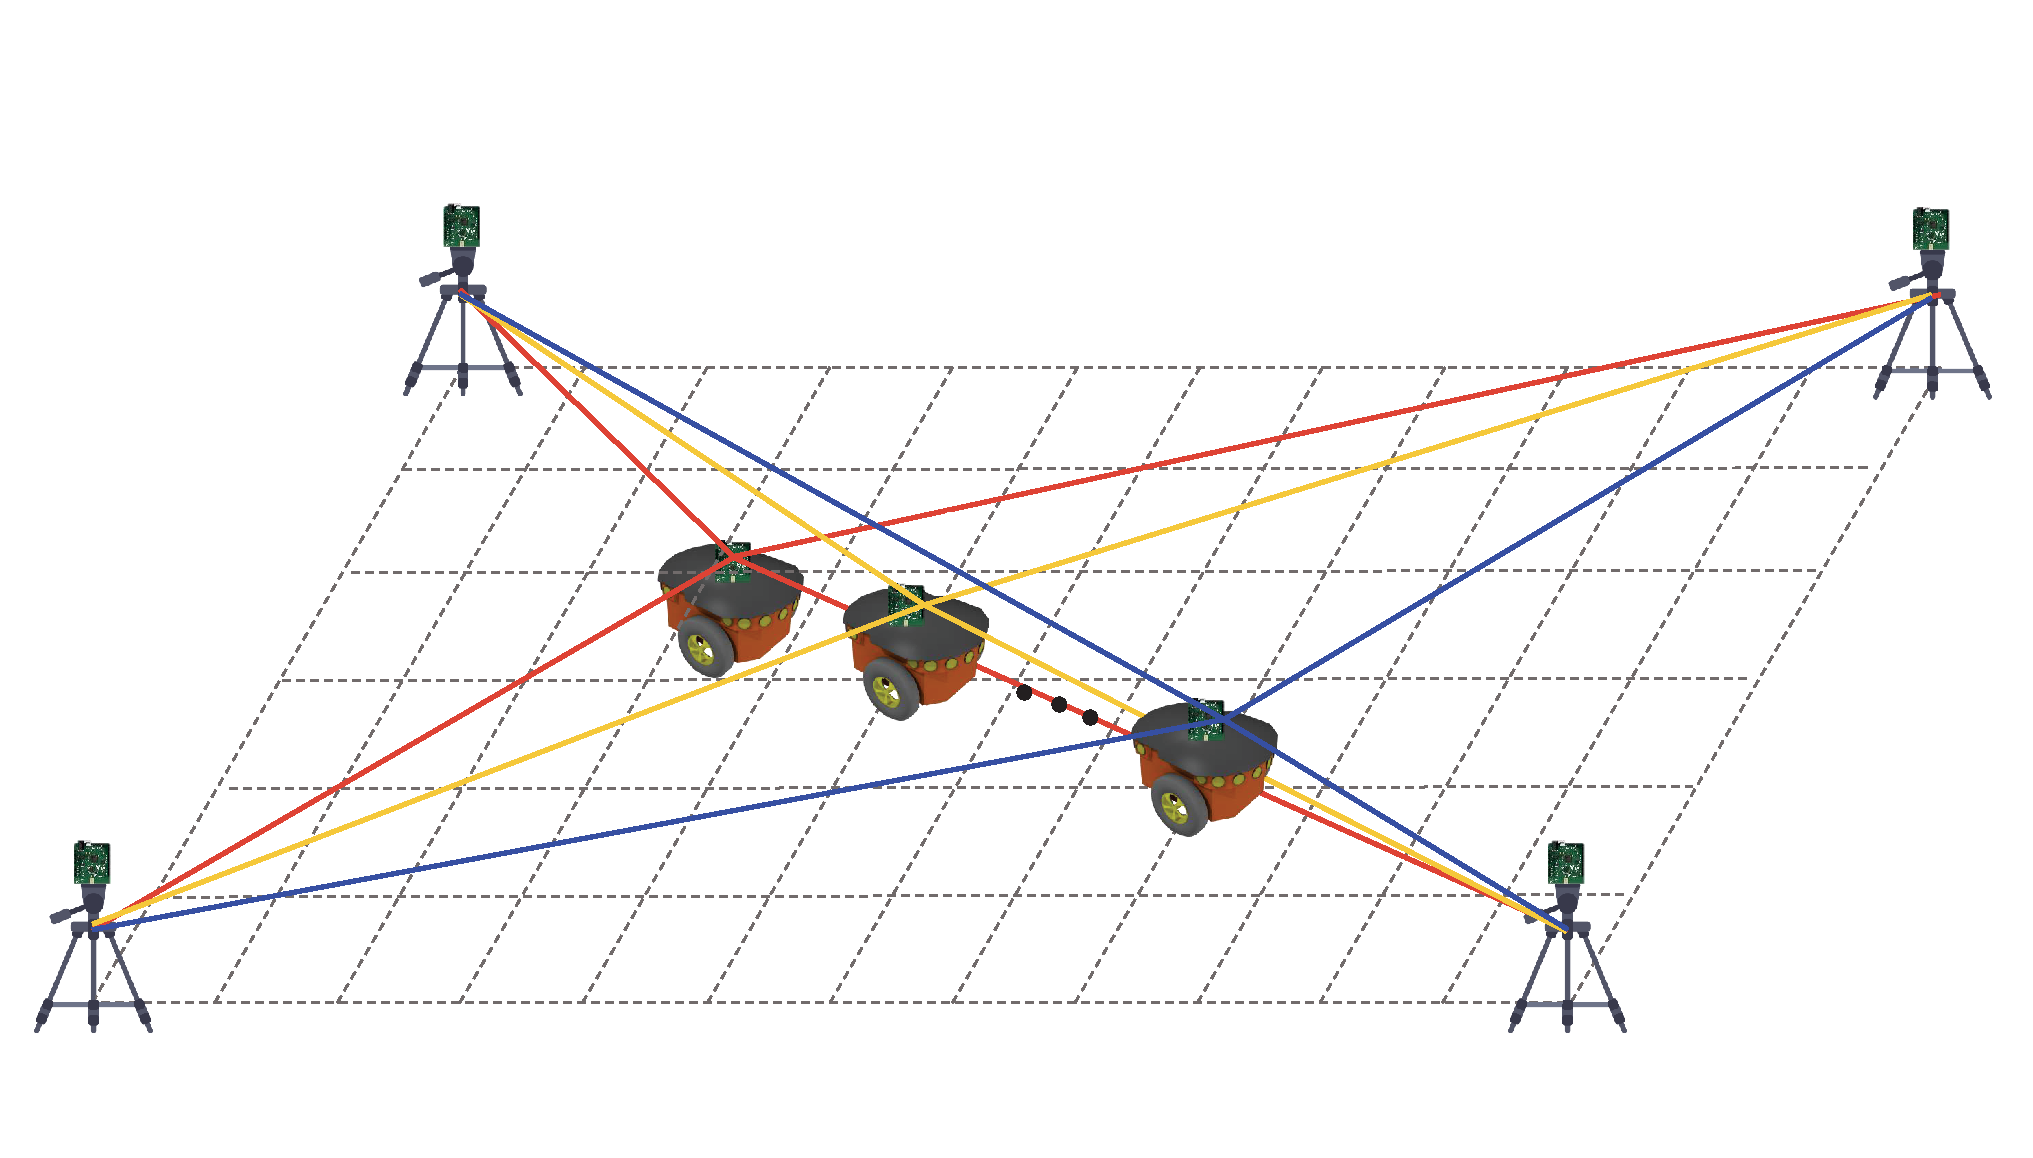
\includegraphics[trim={0 0 0 1cm}height=4.5cm]{IROS2018_image_1}
	\label{fig:example}
	%	}
	
	\caption{Overall architecture of multimodal stacked Bi-LSTM. }
	
\end{figure*}


\subsubsection{Localization with Deep Learning}
There have been many approaches combining Simultaneous Localization and Mapping (SLAM) with deep learning, aiming to overcome the limitations on SLAM only technique such as difficulty on tuning the proper parameters in different environments and recovering an exact scale. Actually, those researches are showing the superior performance to the traditional SLAM approaches.


One of the popular SLAM techniques with deep learning is CNN-SLAM \cite{tateno2017cnn} which takes Convolutional Neural Networks (CNNs) to precisely predict the depth from a single image without any scene-based assumptions or geometric constraints, allowing them to recover the absolute scale of reconstruction. Another approach using deep learning for localization is Deep VO \cite{clark2017vinet} In this method, Recurrent Convolutional Neural Networks (RCNNs) is utilized. Specifically, feature representation is learned by Convolutional Neural Networks and Sequential information and motion dynamics are obtained by deep Recurrent Neural Networks without using any module in the classic VO pipeline.



\subsubsection{Applications of LSTMs}

There are many variations of LSTM architecture. As studies of deep learning are getting popular, various modified architectures of LSTM have been proposed for many tasks in a wide area of science and engineering. Because LSTM is powerful when dealing with sequential data and infering output by using previous inputs, LSTM is utilized to estimate pose by being attached to the end part of deep learning architecture \cite{wang2017deepvo, kendall2015posenet, turan2018deep}  as a stacked form of LSTM. In addition, LSTM takes many various data as input; LSTM is exploited for sequential modeling using LiDAR scan data \cite{gladh2016deep}, images \cite{walch2017image, wang2017deepvo}, IMU \cite{ordonez2016deep}, a fusion of IMU and images \cite{clark2017vinet}. \textcolor{red}{Since existing RO-SLAM performs localization using low-dimensional data, it is difficult to estimate even if the value deviates slightly from the model. In addition, LSTM has the advantage of being able to solve long-term dependence problem of traditional RNN, and it is possible to model it by non-linear mapping through analyzing the current situation without modeling data characteristics separately. Therefore, we propose RO SLAM technology using deep learning based SLAM which applies the advantages of LSTM and deep learning to solve the disadvantages of RO SLAM.}


\section{Our approaches}

In this chapter, we introduce our proposed neural network model which is used for estimating the robot’s pose and Landmarks’ position when only the range sensor data is given from each distance sensor. Firstly, the overall network architecture \textcolor{red}{is} provided. Then, the details of each part \textcolor{red}{are} explained.   

\subsection{Network Architectures}

As it is illustrated in Fig. 2, our proposed stacked Bi-LSTM \textcolor{red}{can be divided} into 3 parts: (1) Input part, which accepts and \textcolor{red}{preprocesses} the sequences of the \textcolor{red}{sensors} with multiple bidirectional LSTM layers. (2) Hidden layer part consisting of attention modules and bidirectional LSTM layer (3) Output part where a fully-connected output layer gives Robot’s pose and \textcolor{red}{positions} of landmarks as \textcolor{green}{the network's final} results. 

\subsection{Multimodal LSTM}

\textcolor{green}{To} effectively accept the \textcolor{red}{inputs} collected from the multiple sensors, instead of \textcolor{green}{using a single layer} as an input layer, we use \textcolor{green}{several} LSTM layers, thinking that each single sensor represents a different modality. Each layer corresponds to the input of each distance sensor. In other words, if N sensors are used for measuring the distance of the robot, the number of input layers also would be N. \textcolor{green}{And,} the MTh layer accepts an input from the MTh sensor. \textcolor{green}{So, the network is able to represent total N modalities.} By doing so, we can further expect that the input layers \textcolor{green}{can} act as the sensor calibration process in traditional RO-SLAM, allowing the sensors to be tuned respectively with the input layer’s parameters.

\subsection{Bidirectional LSTM}

As traditional RO-SLAM \cite{blanco2008pure,blanco2008efficient} takes an odometry which is an accumulated data from the beginning to the present point, our network takes sensor data for the time period l. So, if the current time stamp is t, the input layers take the sensor data obtained from timestamp \textcolor{green}{t-l+1} to t. \textcolor{green}{For dealing with such sequential information, LSTM network which is one of the most appropriate network for sequential data is applied to our network and each LSTM layer is designed to have l cells.} Furthermore, to take \textcolor{red}{an} advantage from the bidirectional time flow, normal time order and reverse time order, we \textcolor{green}{place the bidirectional LSTM layers in the three different locations. Each bidirectional LSTM layer} consists of 2 independent LSTM layers corresponding to normal and reverse time order repectively. Individual LSTM layers play a different role. The LSTM layers of input part take and preprocess the sequence of sensor data. LSTM layer placed between input and output layer takes a spatial information from a previous spatial attention layer and send it to another temporal Attention layer. Lastly, \textcolor{green}{the LSTM layer at the end outputs the positions of robot and landmars.}

\subsection{Attention layer}

To precisely estimate the Robot’s pose and landmarks’ position, it is important for the network to distinguish which is more meaningful information and which is less \textcolor{green}{for preventing} to focus on less significant information. So, we add the two different types of attention modules \cite{luong2015effective} which extract something more important and related to the task information \textcolor{green}{by making the network to focus on different part of input sequence}. \textcolor{green}{The first attention modules placed between the input LSTM layers and the second LSTM layer are called “Spatial attention modules“. The spatial attention modules are represented as blue blocks in Fig. 2.} These attention modules can judge \textcolor{green}{which sensor has more spatial information.} The second attention \textcolor{red}{modules} corresponding to the red blocks in Fig. 2 \textcolor{red}{are} the \textcolor{green}{"Temporal attention modules". These temporal attention modules can determine which time stamp has more useful information about time,} allowing the network to attend that time stamp more.  

\subsection{Stacked Architecture}

In deep learning, the number of layers stacked is getting large, intending to increase the non-linearity and correspondingly to improve the performance. Likewise, the multiple LSTM layers can be stacked as well \cite{dyer2015transition}, enabling more complex representation and higher performance. In stacked Bi-LSTM, total 3 LSTM layers are stacked in the series. 


\section{Experiment}


\subsection{Experimental environment} 

 \textcolor{blue}{Our experimental system consists of a UWB(ultra wideband) sensor tag and eight anchors that have a UWB transceiver, the motion capture system with 12 cameras, a mobile robot and a small form-factor computer. UWB sensor anchors attached to landmarks become the end points of the range measurements. The anchors transmit the UWB signal. A UWB sensor tag attached to a robot becomes the opposite side end point of the measurements. The tag receives the signal and measures the range between two devices. Each UWB transceiver, DW1000 UWB-chip made by Decawave, supports 6 RF bands from 3.5 GHz to 6.5 GHz. It measures in centimeter-level accuracy . The motion capture system is Eagle Digital Realtime system of motion analysis corporation that operates with the principle of stereo pattern recognition that is a kind of photogrammetry based on the epipolar geometry and the triangulation methodology. The system has < 1mm accuracy. A mobile robot used in experiment is iClebo Kobuki from Yujinrobot that has 70 cm/s maximum velocity . The small form-factor computer is a gigabyte Ultra compact PC. Deep learning framework used for our network is pytorch 0.4.0 on python 3.6. The network inferences on the same setting.
 Fig. \ref{setting} shows the description of experimental environment. The UWB tag is attached to mobile robot that has a small compact computer. The UWB anchors are attached to stands that have two different heights. The anchors are positioned randomly in the square space. Inside of the space, a mobile robot goes on various random paths by experimenters. During the robot is going on, the data is saved in the computer. The distance data used for input data is measured by the UWB sensors. The global position data used for ground truth is measured by the motion capture system. After time synchronizing these two kinds of data, these are paired in a dataset. Each path has one dataset. All the paths are different.}

\begin{figure}[h]
	\centering
	\begin{subfigure}[b]{.25\textwidth}
		\centering
		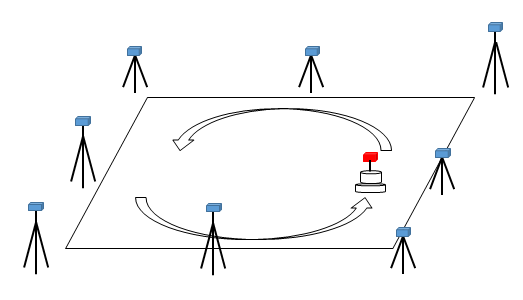
\includegraphics[width=.9\textwidth]{descriptionSystem}
		\label{setting:sub1} 	
		\caption{Description.}
	\end{subfigure}%
	\begin{subfigure}[b]{.25\textwidth}
		\centering
		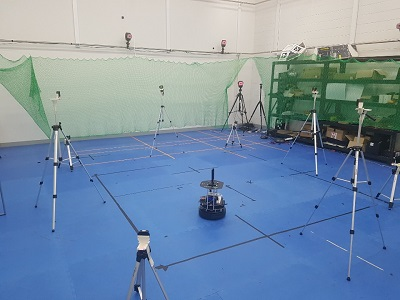
\includegraphics[width=.9\textwidth]{actualSystem}
		\label{setting:sub2} 	
		\caption{Actual.}
	\end{subfigure}
	\caption{Experimental system overview. In (a), anchors are attached to landmarks. A tag is attached to a mobile robot. The robot goes on random paths in square space. (b) shows actual experiment situation.}
	\label{setting}
\end{figure}

\subsection{Training/Test Dataset}

 \textcolor{blue}{In the computer there are two different thread. One receives UWB sensor data. The other one receives global position data. To synchronize time, we make an independent thread that concatenates and saves these data at the same time. The data is saved at 20Hz frequency. The description is shown in Fig. \ref{fig:sync}. After the experiment, we separate the entire dataset to two types, some are the training datasets and others are test datasets.}

\begin{figure}[h]
	\centering
	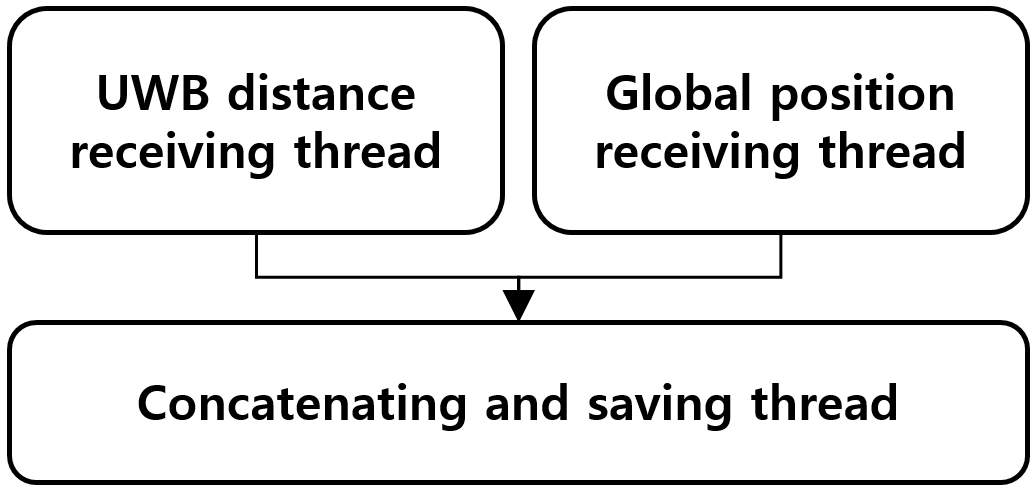
\includegraphics[width=.9\linewidth]{figure2}
	\caption{\textcolor{red}{Data syncronizing method. UWB distance data and the global position data are received to different thread. To syncronize time, another independent thread concatenates and saves these two kinds of data.}}
	\label{fig:sync}
\end{figure}

\subsection{Sensor calibration}
 \textcolor{red}{In addition, to use the distance data for traditional RO-slam we should calibrate the distance from each anchors. To calibrate it, we follow the method in the baseline paper.} \textcolor{blue}{As you can see in Fig. \ref{calibration}(a), we measure the data from a tag to each anchors at the points where the actual distance was measured by 1m, 2m, 3m, 4m. Fig. \ref{calibration}(b) shows that four different anchors are measured at the same time.} By using the linear regression, we compute the ratio between the measurement and the actual distance. And the ratios of each anchor are used to calibrate it.

\begin{figure}[h]
	\centering
	\begin{subfigure}[b]{.35\textwidth}
		\centering
		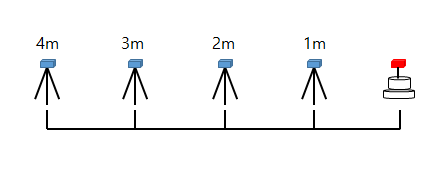
\includegraphics[width=.9\textwidth]{calib}
		\label{calibration:sub1} 	
		\caption{}
	\end{subfigure}%
	\begin{subfigure}[b]{.15\textwidth}
		\centering
		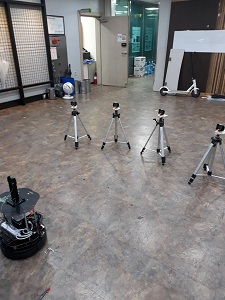
\includegraphics[width=0.9\textwidth]{calib2}
		\label{calibration:sub2} 	
		\caption{}
	\end{subfigure}
	\caption{Sensor calibration overview. (a) shows The formation between a tag and an anchor. (b) shows that four anchors are measured at the same time.}
	\label{calibration}
\end{figure} 

\subsection{Training Loss}
The network is programmed by Tensorflow, which is deep learning library of python trained by using a GTX 1080 Ti and GTX Titan. The Adam optimizr is exploited to train the network during 1000 epochs with 0.0002 learning rate, 0.7 decay rate, and 5 decay step. Besides, Dropout is introduced to prevent the models from overfitting. 

Let $\Theta$ be the parameters of our RNN model, then our final goal is to find optimal parameters $\Theta^{*}$ for localization by minimizing Mean Square Error (MSE) of Euclidean distance between ground truth position $Y_k$ and estimated position $\hat{Y_k}$.

\begin{equation}
\Theta^{*} = \underset{\Theta}{\mathrm{argmin}} \sum_{k=1}^N \parallel Y_k - \hat{Y_k} \parallel^{2}
\end{equation}  

\section{Results}

 \textcolor{green}{To verify our proposal that RNNs can estimate the robot's position through varying range data, we trained our RNN-based multimodal architecture. Plus, to compare to previous traditional SLAM algorithm, we also estimate robot's position by particle filter(PF) based algorithm.}

 As illustrated in Experiment session, train data are our own data gathered by UWB sensors and motion capture camera, so neural networks take range-only measurements as input and output robot's position. Ground truth data is robot's position measured by eagle eye motion capturer, whose error is in mm units. The results of trajectory prediction are shown in Fig. \ref{fig:trajectory} and Root-Mean-Squared Error (RMSE) are shown in Table \ref{RMSE_table}.

 We set two test trajectory cases. However, unexpectedly, it was uncertain to say that which algorithm has better performance. In case of test1, Performance of PF based localization is better than performance of our architecture, whereas performance of RNN-based neural networks architecture is better in case of test2. 
 
 We analyzed the reason why our multimodal architecture is less accurate. First of all, We investigate distance error graph with time step, as shown in \ref{fig:error}. The graph indicates that our deep learning based RNN architecture have a tendency that sometimes it estimates wrong position that is far from the Ground truth. So we conclude that it is because train data is too small to infer position correctly. Due to little amount of train data that only just consist of 11258 time step, it is insufficient to cover all possible 3D space where robot can explore. Because neural networks infer outputs based on train data, neural networks do not estimate the space where is not included in train data. 
 
 
 \begin{figure*}[h]
 	\centering
 	\begin{subfigure}[b]{.50\textwidth}
 		\centering
 		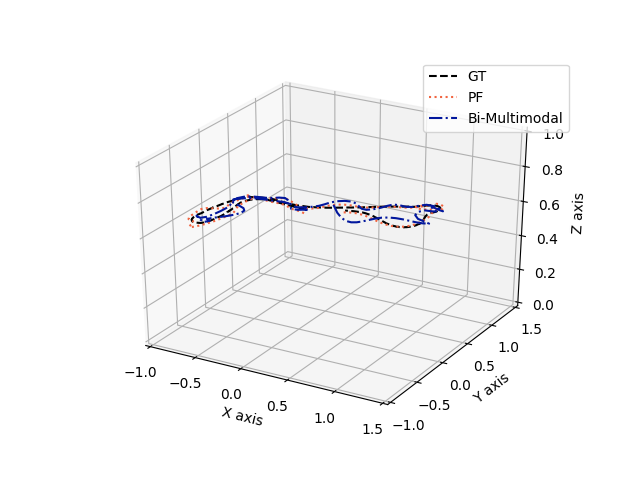
\includegraphics[width=.9\textwidth]{PF_multimodal_comparison2}
 		\label{fig:trajectory1} 	
 		\caption{}
 	\end{subfigure}%
 	\begin{subfigure}[b]{.50\textwidth}
 		\centering
 		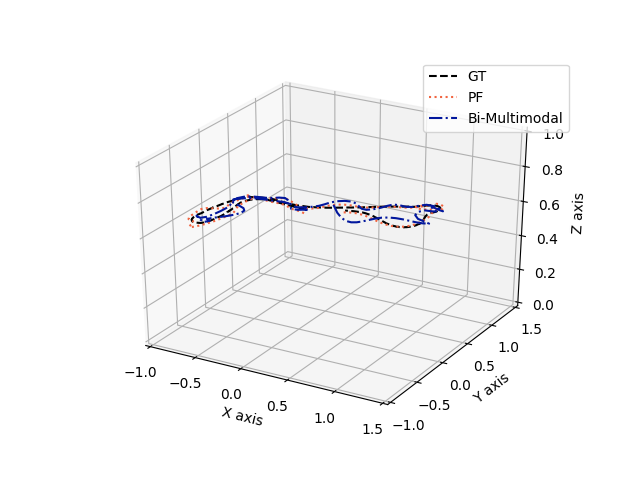
\includegraphics[width=0.9\textwidth]{PF_multimodal_comparison2}
 		\label{fig:trajectory2} 	
 		\caption{}
 	\end{subfigure}
 	\caption{Trajectories estimated by particle filter-based algorithm and our neural networks' architecture. (a)A trajectory of test1 data (b)A trajectory of test2 data}
 	\label{fig:trajectory}
 \end{figure*} 
 
 \begin{figure*}[h]
 	\centering
 	\begin{subfigure}[b]{.50\textwidth}
 		\centering
 		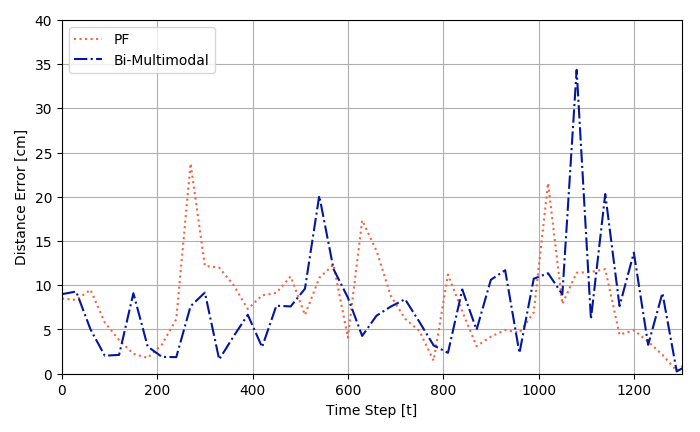
\includegraphics[width=.9\textwidth]{PF_multimodal_error1}
 		\label{fig:error1} 	
 		\caption{}
 	\end{subfigure}%
 	\begin{subfigure}[b]{.50\textwidth}
 		\centering
 		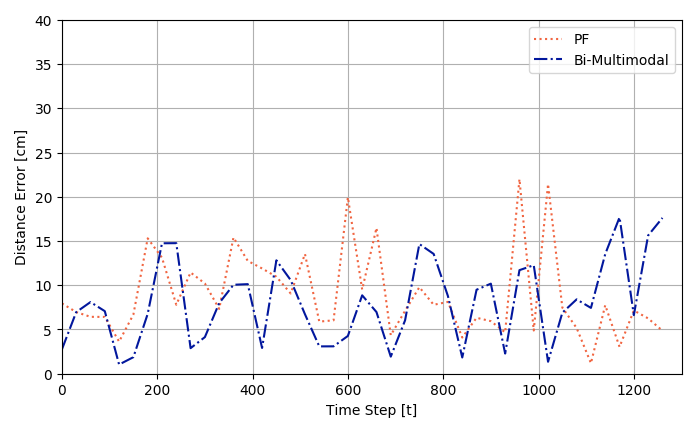
\includegraphics[width=0.9\textwidth]{PF_multimodal_error2}
 		\label{fig:error2} 	
 		\caption{}
 	\end{subfigure}
 	\caption{The distance error graphes with time step. (a) The Distance error of test 1 data  and (b)distance error of test 2 data}
 	\label{fig:error}
 \end{figure*} 
  
 Secondly, we realized that many articles about estimating position using deep learning architecture tend to generate grid maps to reduce error caused by the noise of that neural networks, but our neural networks output float directly. As shown in Fig. \ref{fig:error}. 
 
 Therefore, we can conclude that the performance improves as the non-linearity of the architecture increases.
 
 
\begin{table}[h]
	\centering
	\begin{tabular}{cclcl}
		\hline
		\multicolumn{5}{c}{The results of RMSE{[}cm{]}}                                                                  \\ \hline
		\multicolumn{1}{c|}{Model}                    & \multicolumn{2}{c|}{Test1} & \multicolumn{2}{c}{Test2}      \\ \hline
		\multicolumn{1}{c|}{Particle filter-based}    & \multicolumn{2}{c|}{\textbf{9.1827}}     & \multicolumn{2}{c}{9.8803}          \\
		\multicolumn{1}{c|}{Bidirectional Multimodal} & \multicolumn{2}{c|}{11.3301}     & \multicolumn{2}{c}{\textbf{9.7528}}
	\end{tabular}
	\caption{Root mean squared error of each case}
	\label{RMSE_table}
\end{table}


\section{Conclusion}

In this paper, we proposed a novel approach to range-only SLAM using multimodal-based RNN models and tested our architectures in two test data.

Using deep learning, our structure directly learns the end-to-end mapping between distance data and robot position. The multimodal bidirectional stacked LSTM structure exhibits the precise estimates of robot positions, but some cases, it is less accurate than traditional SLAM algorithm. Therefore, we could check the possibility that our multimodal LSTM-based structure can substitute traditional algorithms if we make our train data more sufficient. 

As a future work, because train dataset is insufficient, the proposed method needs to be tested in more-rich train data situation. Besides, we will modify end parts of our neural networks architecturethe utilizing generating grid maps to check whether RNNs can deal with the rank-deficient range only measurements well.

\bibliographystyle{IEEEtran}
% argument is your BibTeX string definitions and bibliography database(s)
\bibliography{./IEEEabrv,./MyBib}


\end{document}
